\documentclass [11pt]{articleSBPO}

\usepackage[brazil]{babel}
\usepackage[utf8]{inputenc}
\usepackage[T1]{fontenc}
\usepackage{graphics}
\usepackage[a4paper,top=3.3cm,left=2.9cm,right=2.9cm,bottom=2.5cm,noheadfoot]{geometry}
\usepackage{algorithm}
\usepackage{algorithmic}
\usepackage{times}
\usepackage{amsmath}
\usepackage{amssymb}
\usepackage{setspace}
\usepackage{graphicx}
\usepackage{subfig}
\usepackage{indentfirst}
\usepackage{icomma}
\usepackage{url}
\usepackage{longtable}
\usepackage{lscape}
\usepackage{array}
\usepackage[alf]{abntex2cite}
\usepackage{epstopdf}
\usepackage{rotating}
\newcommand{\up}[1]{\raisebox{1.3ex}[0pt]{#1}}
% \usepackage{latex8}
\floatname{algorithm}{Algoritmo}
\def\figurename{Figura}
\def\tablename{Tabela}

%%%%%%%%%%%%%%%%%%%%%%%%%%%%%%%%%%%%%%%%%%%%%%
%     configurações do pacote algorithm
%%%%%%%%%%%%%%%%%%%%%%%%%%%%%%%%%%%%%%%%%%%%%
% \renewcommand{\algorithmcfname}{alg}
\floatname{algorithm}{Algoritmo}
\renewcommand{\algorithmicrequire}{\textbf{Entrada:}}
\renewcommand{\algorithmicensure}{\textbf{Saída:}}
\renewcommand{\algorithmicend}{\textbf{fim}}
\renewcommand{\algorithmicif}{\textbf{se}}
\renewcommand{\algorithmicthen}{\textbf{então}}
\renewcommand{\algorithmicelse}{\textbf{senão}}
\renewcommand{\algorithmicelsif}{\algorithmicelse\ \algorithmicif}
\renewcommand{\algorithmicendif}{\algorithmicend\ \algorithmicif}
\renewcommand{\algorithmicfor}{\textbf{para}}
% \renewcommand{\algorithmicto}{\textbf{até}}
\renewcommand{\algorithmicforall}{\textbf{para todo}}
\renewcommand{\algorithmicdo}{\textbf{faça}}
\renewcommand{\algorithmicendfor}{\algorithmicend\ \algorithmicfor}
\renewcommand{\algorithmicwhile}{\textbf{enquanto}}
\renewcommand{\algorithmicendwhile}{\algorithmicend\ \algorithmicwhile}
\renewcommand{\algorithmicloop}{\textbf{laço}}
\renewcommand{\algorithmicendloop}{\algorithmicend\ \algorithmicloop}
\renewcommand{\algorithmicrepeat}{\textbf{repita}}
\renewcommand{\algorithmicuntil}{\textbf{até que}}
\renewcommand{\algorithmicprint}{\textbf{imprima}}
\renewcommand{\algorithmicreturn}{\textbf{retorne}}
\renewcommand{\algorithmictrue}{\textbf{verdadeiro}}
\renewcommand{\algorithmicfalse}{\textbf{falso}}
\renewcommand{\algorithmicnot}{\textbf{não}}

%%%%%%%%%%%%%%%%%%%%%%%%%%%%%%%%%%%%%%%%%%%%%%%%%%%%%%%%%%%%%%%%%%%%%%%%%%%%%%%%%%%%%%%%%%%%%%

%\usepackage{attrib}

%\usepackage{natbib} % pacote que traz o formato das citações por autor (não por números, que é o default do LaTeX)

\newtheorem{Lemma}{Lemma}
\newtheorem{Theorem}{Theorem}
\newtheorem{Condition}{Condition}

\def\nohyphen{\pretolerance=1000 \tolerance=1000 \hyphenpenalty=1000 \exhyphenpenalty=1000}

\setlength{\parindent}{1.50cm}

\begin{document}
\pagestyle{empty}%tira a numeração das páginas

\thispagestyle{empty}%tira a numeração da página em questão

\begin{center}
%\LARGE{\textbf{\normalsize UMA ABORDAGEM MULTIOBJETIVO INTEIRA MISTA PARA O PROBLEMA DA DIETA EM CRECHES}}
\LARGE{\textbf{\normalsize UMA ABORDAGEM MULTIOBJETIVO PARA O PLANEJAMENTO DE PRODUTOS LATICÍNIOS}}
\end{center}

\vspace{5mm}

\begin{center}
\textbf{Felipe F. Cruz$^{\alpha}$, Thiago H. de M. Mendes$^{\alpha}$, André R. da Cruz$^{\beta}$} \\
Universidade Federal de Viçosa, campus Rio Paranaíba, \\
Rodovia MG-230 Km 7, Rio Paranaíba - MG, Brasil \\
\{felipe.f.cruz, thiago.h.mendes, andre.cruz\}@ufv.br
\par
$\alpha$ Graduando em Sistemas de Informação \\
$\beta$ Instituto de Ciências Exatas e Tecnológicas \\
\end{center}


\begin{center}
{\bf RESUMO}
\end{center}
\nohyphen{ 

\noindent \textbf{PALAVRAS CHAVE. Produtos Laticínios, Planejamento da Produção, Programação Multiobjetivo Linear, Mix de Produtos.} 

\vspace{11pt}

\noindent \textbf{Áreas Principais: ADM – Apoio à Decisão Multicritério, AG\&MA – PO na Agricultura e Meio Ambiente, IND – PO na Indústria.}
}

\begin{center}
{\bf ABSTRACT}
\end{center}
\nohyphen{

\noindent \foreignlanguage{english}{\textbf{KEYWORDS. Dairy Products, Production Planning, Multiobjective Linear Programming, Product Mix.}}

\vspace{11pt}

\noindent \foreignlanguage{english}{\textbf{Main areas: Multicriteria Decision Support, OR in Agriculture and Environment, OR in Industry.}}
}

\newpage %força uma quebra de página

\section{Introdução}\label{sec:introducao}

Após a Revolução Industrial, houve um contínuo crescimento de organizações pelo mundo, fazendo com que as pequenas oficinas de artesãos dessem lugar a grandes organizações com variados setores, o que agregou complexidade de produção de produtos. Devido a essa complexidade surgiu a Pesquisa Operacional (PO), que segundo \cite{hillier; lieberman, 2013} é aplicada a problemas envolvendo como conduzir e coordenar as operações (isto é, as atividades) em uma organização. A PO abrange diversas áreas como manufatura, transportes, construção, telecomunicações, planejamento financeiro, entre outros. Para se encontrar a melhor solução (solução ótima) de um problema de otimização, um modelo matemático deve ser gerado mantendo as características e restrições do problema.

Para a otimização de um problema em PO, são utilizadas algumas métricas de cálculos para a sua solução. Tais métricas podem ser trabalhosas se executadas manualmente em problemas com muitas variáveis e restrições. Para tal problema, existem algumas ferramentas que resolvem tais problemas de PO, conhecidos como solvers. Alguns desses solvers são o Gurobi da Gurobi Optimization, Inc. (GUROBI, 2014), o Lingo e Lindo da Lindo System, Inc. (LINDO Systems, Inc., 2013, 2014), o GNU Linear Programming Kit GLPK (GNU Project, 2010) e o lpsolve (LPSOLVE, 2015). Outro problema enfrentado em geral por estudantes, é a dificuldade de entender como funcionam os algoritmos usados em PO em um problema. Para isso, existem solvers de fins didáticos tanto acompanhadas de livros de PO como o TORA (TAHA, 2008), quanto disponíveis na web como o PROLIN(DPI-UFV, 2012). 

Existem poucos solvers didáticos gratuitos disponíveis na web que apresentem a resolução detalhada de problemas de Programação Linear (PL) e Programação Linear Inteira (PLI). Grande parte desses solvers não possuem uma interface intuitiva para o usuário ou demandam muito tempo do usuário na inserção de valores de um determinado problema a cada vez que se tem acesso ao sistema.

Este trabalho apresenta o SIMPL(Sistema Interativo para Métodos de Programação Linear), que é um solver didático gratuito disponível na Internet, com o intuito de auxiliar estudantes na compreensão de problemas de PO, utilizando-se dos métodos Branch-and-Bounch (PLI), Métodos Simplex (PL) e de Problemas de Transporte(PL). Através dele, é possível inserir modelos matemáticos a serem solucionados e serem salvos em arquivo TXT. Também apresenta o detalhamento da resolução, visando facilitar o entendimento do usuário dos métodos aplicado ao modelo inserido. O SIMPL foi desenvolvido utilizando as linguagens Javascript, CSS3 e HTML5 e o framework Bootstrap para desenvolvimento da interface. A biblioteca glpk.js foi utilizada para a resolução dos problemas inseridos.

O trabalho está organizado da seguinte forma: a seção \ref{sec:metodos} apresenta uma definição breve e formal dos métodos presentes no solver para resolução de problemas de PL;


\section{Métodos de resolução de Problemas de Programação Linear}
\label{sec:metodos}

\subsection{Método Simplex}

O método Simplex proposto por George Dantzig, é um método matricial para resolver problemas de Programação Linear. Ele executa iterativamente em busca da solução ótima entre as soluções básicas viáveis. 

Na figura 2, é apresentado os passos iterativos do método em busca da solução ótima.

\begin{figure}[!h]
\centering
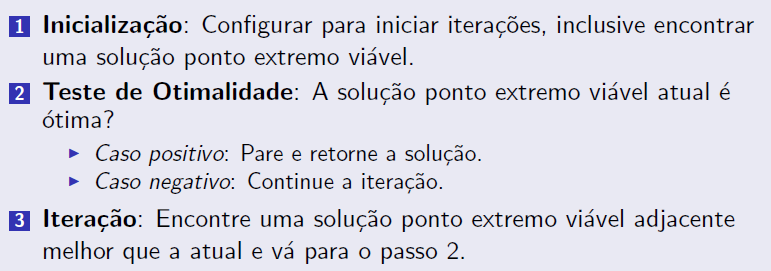
\includegraphics[width=0.5\textwidth]{img/img1.png}
\caption[]{Estrutura iterativa do método}
\label{fig:figura1}
\end{figure}

Em um problema de PL, se houverem restrições que demandem variáveis artificiais, elas são inseridas para formar uma solução inicial semelhante a um problema em que todas as variáveis são de folga. O Simplex Grande M consiste em aplicar grandes punições as variáveis artificiais na função objetivo, fazendo com que essas variáveis tenham valor 0 na solução ótima.

Porém, esses altos valores de M podem gerar grandes erros de arredondamento. O método Duas Fases elimina essa constante M e resolve o método através de duas fases:

. Fase 1: Tenta encontrar uma solução inicial básica. Se achar, passa para a fase 2.
. Fase 2: É chamada para resolver o problema original.

O Simplex generalizado é usado quando a solução básica inicial é não factível e não ótima. Portanto, quando a solução é infactível, usa-se as regras do simplex dual até reestabelecer a viabilidade ou certificar que não existe solução factível. Quando a solução é factível, basta aplicar as regras do simplex primal.

\subsection{Branch-and-Bounch}

A Programação linear inteira mista(PLIM) é uma PL(Programação Linear) que existe alguma ou todas as variáveis não inteiras. Portanto precisamos de encontrar uma nova solução ótima para evitarmos casos de números parciais. Simplesmente com o arredondamento, a solução muitas vezes pode sair da região viável, comprometendo a otimalidade. 

Para resolver usando o Branch and Bound, primeiro resolvemos o problema usando o Relaxamento, o que significa resolvê-lo pelo Simplex Revisado como se não houvesse restriçőes inteiras.

Como o exemplo usado envolve um problema de maximização que engloba todas as soluçőes inteiras, então esse é um limite superior da PLIM. Em seguida, escolhe-se uma variável não inteira. Comumente, escolhe-se a variável mais fracionada, que esteja mais próxima do valor mediano ou mais distante de um número inteiro.

Quando a solução não apresentar mais valores fracionados, então é encontrado a solução ótima inteira. 

\subsection{Problema de Transporte}

O problema de transporte é uma sub-classe de Programação Linear que trata do envio de mercadorias de uma origem a um destino, sendo executada através de uma rota ótima, ou seja, com menor custo, tempo e que satisfaça as restrições de fornecimento e demanda. Tal analogia pode ser abrangida para outras áreas como controle de estoque, programação de empregos, entre outros.

Segundo \cite{TAHA}, O problema geral consiste em m origens e n destinos, cada um representado por um nó, conforme mostra a Figura 2. Os arcos representam o trajeto entre origem e destino. Em um trajeto, são determinadas duas características:

    1) O custo de transporte por unidade em um trajeto;
    2) A quantidade enviada.

O objetivo do problema é determinar essa quantidade enviada ótima, de forma a satisfazer as restrições de demanda e suprimento.

As etapas seguidas pelo algoritmo do problema de transporte são as mesmas presentes no método Simplex.

\begin{figure}[!h]
\centering
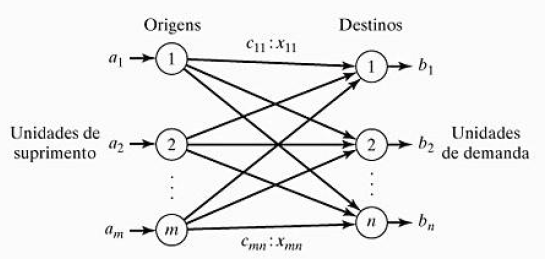
\includegraphics[width=0.5\textwidth]{img/img2.png}
\caption[]{Esquematização do Problema de Transporte}
\label{fig:figura2}
\end{figure}

\subsubsection{Método do canto do Noroeste}

O método do Canto Noroeste consiste em iniciar o método iterativo pela primeira célula da tabela simplex(x11), ou seja, pelo canto Noroeste da tabela.

\subsubsection{Método do menor custo}

O método do menor custo se concentra em rotas mais baratas. Ou seja, ela denota maior peso possível a célula da tabela que tiver o menor valor. Em seguida, tal coluna ou linha selecionada é cancelada e o valores em demanda ou fornecimento é reajustado.

Se houver uma linha e uma coluna satisfeitas simultaneamente, apenas uma delas será cancelada. Logo após, selecione novamente a célula de menor valor e repita o processo até restar apenas uma linha ou coluna.

\subsubsection{Método de aproximação de Vogel (MAV)}

Segundo \cite{TAHA}, o MAV é uma versão melhorada do método de menor custo, que em geral, produz soluções iniciais melhores.

\section{Resultados}
\label{sec:resultados}

\bibliography{referencias}
\bibliographystyle{abnt-alf}

\end{document}